% Options for packages loaded elsewhere
\PassOptionsToPackage{unicode}{hyperref}
\PassOptionsToPackage{hyphens}{url}
%
\documentclass[
]{article}
\usepackage{amsmath,amssymb}
\usepackage{iftex}
\ifPDFTeX
  \usepackage[T1]{fontenc}
  \usepackage[utf8]{inputenc}
  \usepackage{textcomp} % provide euro and other symbols
\else % if luatex or xetex
  \usepackage{unicode-math} % this also loads fontspec
  \defaultfontfeatures{Scale=MatchLowercase}
  \defaultfontfeatures[\rmfamily]{Ligatures=TeX,Scale=1}
\fi
\usepackage{lmodern}
\ifPDFTeX\else
  % xetex/luatex font selection
\fi
% Use upquote if available, for straight quotes in verbatim environments
\IfFileExists{upquote.sty}{\usepackage{upquote}}{}
\IfFileExists{microtype.sty}{% use microtype if available
  \usepackage[]{microtype}
  \UseMicrotypeSet[protrusion]{basicmath} % disable protrusion for tt fonts
}{}
\makeatletter
\@ifundefined{KOMAClassName}{% if non-KOMA class
  \IfFileExists{parskip.sty}{%
    \usepackage{parskip}
  }{% else
    \setlength{\parindent}{0pt}
    \setlength{\parskip}{6pt plus 2pt minus 1pt}}
}{% if KOMA class
  \KOMAoptions{parskip=half}}
\makeatother
\usepackage{xcolor}
\usepackage[margin=1in]{geometry}
\usepackage{color}
\usepackage{fancyvrb}
\newcommand{\VerbBar}{|}
\newcommand{\VERB}{\Verb[commandchars=\\\{\}]}
\DefineVerbatimEnvironment{Highlighting}{Verbatim}{commandchars=\\\{\}}
% Add ',fontsize=\small' for more characters per line
\usepackage{framed}
\definecolor{shadecolor}{RGB}{248,248,248}
\newenvironment{Shaded}{\begin{snugshade}}{\end{snugshade}}
\newcommand{\AlertTok}[1]{\textcolor[rgb]{0.94,0.16,0.16}{#1}}
\newcommand{\AnnotationTok}[1]{\textcolor[rgb]{0.56,0.35,0.01}{\textbf{\textit{#1}}}}
\newcommand{\AttributeTok}[1]{\textcolor[rgb]{0.13,0.29,0.53}{#1}}
\newcommand{\BaseNTok}[1]{\textcolor[rgb]{0.00,0.00,0.81}{#1}}
\newcommand{\BuiltInTok}[1]{#1}
\newcommand{\CharTok}[1]{\textcolor[rgb]{0.31,0.60,0.02}{#1}}
\newcommand{\CommentTok}[1]{\textcolor[rgb]{0.56,0.35,0.01}{\textit{#1}}}
\newcommand{\CommentVarTok}[1]{\textcolor[rgb]{0.56,0.35,0.01}{\textbf{\textit{#1}}}}
\newcommand{\ConstantTok}[1]{\textcolor[rgb]{0.56,0.35,0.01}{#1}}
\newcommand{\ControlFlowTok}[1]{\textcolor[rgb]{0.13,0.29,0.53}{\textbf{#1}}}
\newcommand{\DataTypeTok}[1]{\textcolor[rgb]{0.13,0.29,0.53}{#1}}
\newcommand{\DecValTok}[1]{\textcolor[rgb]{0.00,0.00,0.81}{#1}}
\newcommand{\DocumentationTok}[1]{\textcolor[rgb]{0.56,0.35,0.01}{\textbf{\textit{#1}}}}
\newcommand{\ErrorTok}[1]{\textcolor[rgb]{0.64,0.00,0.00}{\textbf{#1}}}
\newcommand{\ExtensionTok}[1]{#1}
\newcommand{\FloatTok}[1]{\textcolor[rgb]{0.00,0.00,0.81}{#1}}
\newcommand{\FunctionTok}[1]{\textcolor[rgb]{0.13,0.29,0.53}{\textbf{#1}}}
\newcommand{\ImportTok}[1]{#1}
\newcommand{\InformationTok}[1]{\textcolor[rgb]{0.56,0.35,0.01}{\textbf{\textit{#1}}}}
\newcommand{\KeywordTok}[1]{\textcolor[rgb]{0.13,0.29,0.53}{\textbf{#1}}}
\newcommand{\NormalTok}[1]{#1}
\newcommand{\OperatorTok}[1]{\textcolor[rgb]{0.81,0.36,0.00}{\textbf{#1}}}
\newcommand{\OtherTok}[1]{\textcolor[rgb]{0.56,0.35,0.01}{#1}}
\newcommand{\PreprocessorTok}[1]{\textcolor[rgb]{0.56,0.35,0.01}{\textit{#1}}}
\newcommand{\RegionMarkerTok}[1]{#1}
\newcommand{\SpecialCharTok}[1]{\textcolor[rgb]{0.81,0.36,0.00}{\textbf{#1}}}
\newcommand{\SpecialStringTok}[1]{\textcolor[rgb]{0.31,0.60,0.02}{#1}}
\newcommand{\StringTok}[1]{\textcolor[rgb]{0.31,0.60,0.02}{#1}}
\newcommand{\VariableTok}[1]{\textcolor[rgb]{0.00,0.00,0.00}{#1}}
\newcommand{\VerbatimStringTok}[1]{\textcolor[rgb]{0.31,0.60,0.02}{#1}}
\newcommand{\WarningTok}[1]{\textcolor[rgb]{0.56,0.35,0.01}{\textbf{\textit{#1}}}}
\usepackage{graphicx}
\makeatletter
\def\maxwidth{\ifdim\Gin@nat@width>\linewidth\linewidth\else\Gin@nat@width\fi}
\def\maxheight{\ifdim\Gin@nat@height>\textheight\textheight\else\Gin@nat@height\fi}
\makeatother
% Scale images if necessary, so that they will not overflow the page
% margins by default, and it is still possible to overwrite the defaults
% using explicit options in \includegraphics[width, height, ...]{}
\setkeys{Gin}{width=\maxwidth,height=\maxheight,keepaspectratio}
% Set default figure placement to htbp
\makeatletter
\def\fps@figure{htbp}
\makeatother
\setlength{\emergencystretch}{3em} % prevent overfull lines
\providecommand{\tightlist}{%
  \setlength{\itemsep}{0pt}\setlength{\parskip}{0pt}}
\setcounter{secnumdepth}{5}
\usepackage{booktabs}
\ifLuaTeX
  \usepackage{selnolig}  % disable illegal ligatures
\fi
\usepackage{bookmark}
\IfFileExists{xurl.sty}{\usepackage{xurl}}{} % add URL line breaks if available
\urlstyle{same}
\hypersetup{
  pdftitle={Survey Data Analysis Report: Influence of Background Music on Study Performance (Enhanced)},
  pdfauthor={Group 39},
  hidelinks,
  pdfcreator={LaTeX via pandoc}}

\title{Survey Data Analysis Report: Influence of Background Music on
Study Performance (Enhanced)}
\author{Group 39}
\date{June 26, 2025}

\begin{document}
\maketitle

{
\setcounter{tocdepth}{2}
\tableofcontents
}
\section{Introduction}\label{introduction}

\subsection{Research Questions}\label{research-questions}

\begin{itemize}
\tightlist
\item
  Q1: How does the type of music or silence influence students' focus
  levels?
\item
  Q2: How do music type and focus level together affect task completion
  time?
\item
  Q3: How does the type of background music impact the time required to
  complete a task?
\end{itemize}

\subsection{Survay Questions}\label{survay-questions}

In this report, we want to analyze whether the genre of background music
has an impact on students' study performance. The hypothesis is that
studying with low-tempo instrumental music helps complete comprehension
tasks more accurately and quickly compared to studying with lyrical
music or in silence. To test this, we have prepared three survey
questions as follows:

\begin{itemize}
\tightlist
\item
  Q1: Type of background music while studying (None, Instrumental, Music
  with lyrics, Other).
\item
  Q2: Focus level while studying with preferred music (1 to 10 scale).
\item
  Q3: Time to complete a typical comprehension assignment (in minutes).
\end{itemize}

This enhanced analysis uses R for data cleaning, comprehensive
exploratory data analysis (EDA), descriptive inference, analytic
inference, and crucial assumption checks for statistical tests. Key R
packages used include \texttt{dplyr}, \texttt{ggplot2}, \texttt{knitr},
\texttt{readxl}, \texttt{car}, \texttt{ggpubr}, and \texttt{broom}.

\section{Data Cleaning}\label{data-cleaning}

The dataset, is in Exel format (\texttt{group39.xlsx}), contains
demographic and survey responses. Data cleaning steps address
inconsistencies, missing values, and outliers.

\begin{itemize}
\tightlist
\item
  \textbf{Renaming Columns:} Columns are renamed for clarity (e.g.,
  DemographicAnswer.1 to Gender, Answer.1 to MusicType).
\item
  \textbf{Handling Missing Values:} Rows with missing \texttt{MusicType}
  are removed, as this is critical for RQ1.
\item
  \textbf{Outlier Removal:} For \texttt{TimeToComplete} (Q3), extreme
  values (e.g., 99999999 minutes) are treated as outliers and removed.
  Values above 360 minutes (6 hours) are considered unrealistic for a
  typical assignment. This helps ensure the statistical analysis is not
  skewed by erroneous entries.
\item
  \textbf{Type Conversion:} \texttt{FocusLevel} (Q2) is converted to
  numeric, and \texttt{TimeToComplete} is cleaned to handle non-numeric
  entries.
\end{itemize}

\begin{Shaded}
\begin{Highlighting}[]
\FunctionTok{library}\NormalTok{(readxl)}
\FunctionTok{library}\NormalTok{(dplyr)}
\NormalTok{data }\OtherTok{\textless{}{-}} \FunctionTok{read\_excel}\NormalTok{(}\StringTok{"group39.xlsx"}\NormalTok{)}

\CommentTok{\# renaming columns}
\NormalTok{data }\OtherTok{\textless{}{-}}\NormalTok{ data }\SpecialCharTok{\%\textgreater{}\%}
  \FunctionTok{rename}\NormalTok{(}\AttributeTok{Gender =}\NormalTok{ DemographicAnswer}\FloatTok{.1}\NormalTok{,}
         \AttributeTok{Age =}\NormalTok{ DemographicAnswer}\FloatTok{.2}\NormalTok{,}
         \AttributeTok{Education =}\NormalTok{ DemographicAnswer}\FloatTok{.3}\NormalTok{,}
         \AttributeTok{MusicType =}\NormalTok{ Answer}\FloatTok{.1}\NormalTok{,}
         \AttributeTok{FocusLevel =}\NormalTok{ Answer}\FloatTok{.2}\NormalTok{,}
         \AttributeTok{TimeToComplete =}\NormalTok{ Answer}\FloatTok{.3}\NormalTok{)}

\CommentTok{\# removing the rows which has missing MusicType}
\NormalTok{data }\OtherTok{\textless{}{-}}\NormalTok{ data }\SpecialCharTok{\%\textgreater{}\%} \FunctionTok{filter}\NormalTok{(}\SpecialCharTok{!}\FunctionTok{is.na}\NormalTok{(MusicType))}

\CommentTok{\# converting focusLevel to numeric}
\NormalTok{data}\SpecialCharTok{$}\NormalTok{FocusLevel }\OtherTok{\textless{}{-}} \FunctionTok{as.numeric}\NormalTok{(}\FunctionTok{as.character}\NormalTok{(data}\SpecialCharTok{$}\NormalTok{FocusLevel))}

\CommentTok{\# cleaning TimeToComplete: handling ranges and outliers}
\CommentTok{\# Convert "10{-}15" to "12.5" and then to numeric}
\NormalTok{data}\SpecialCharTok{$}\NormalTok{TimeToComplete }\OtherTok{\textless{}{-}} \FunctionTok{gsub}\NormalTok{(}\StringTok{"10{-}15"}\NormalTok{, }\StringTok{"12.5"}\NormalTok{, data}\SpecialCharTok{$}\NormalTok{TimeToComplete)}
\NormalTok{data}\SpecialCharTok{$}\NormalTok{TimeToComplete }\OtherTok{\textless{}{-}} \FunctionTok{as.numeric}\NormalTok{(}\FunctionTok{as.character}\NormalTok{(data}\SpecialCharTok{$}\NormalTok{TimeToComplete))}

\CommentTok{\# removing extreme outliers }
\NormalTok{data }\OtherTok{\textless{}{-}}\NormalTok{ data }\SpecialCharTok{\%\textgreater{}\%} \FunctionTok{filter}\NormalTok{(TimeToComplete }\SpecialCharTok{\textless{}=} \DecValTok{360} \SpecialCharTok{|} \FunctionTok{is.na}\NormalTok{(TimeToComplete))}
\NormalTok{data }\OtherTok{\textless{}{-}}\NormalTok{ data }\SpecialCharTok{\%\textgreater{}\%} \FunctionTok{filter}\NormalTok{(TimeToComplete }\SpecialCharTok{!=} \DecValTok{999999999} \SpecialCharTok{|} \FunctionTok{is.na}\NormalTok{(TimeToComplete))}

\NormalTok{data}\SpecialCharTok{$}\NormalTok{MusicType }\OtherTok{\textless{}{-}} \FunctionTok{as.factor}\NormalTok{(data}\SpecialCharTok{$}\NormalTok{MusicType)}
\end{Highlighting}
\end{Shaded}

\section{Exploratory Data Analysis}\label{exploratory-data-analysis}

Exploratory Data Analysis examines the distribution of key variables and
their relationships to address RQ1, providing more detailed insights
into the data's characteristics.

\subsection{Distribution of Music
Type}\label{distribution-of-music-type}

A bar plot shows the frequency of each music type.

\begin{Shaded}
\begin{Highlighting}[]
\FunctionTok{library}\NormalTok{(ggplot2)}
\FunctionTok{ggplot}\NormalTok{(data, }\FunctionTok{aes}\NormalTok{(}\AttributeTok{x =}\NormalTok{ MusicType, }\AttributeTok{fill =}\NormalTok{ MusicType)) }\SpecialCharTok{+}
  \FunctionTok{geom\_bar}\NormalTok{() }\SpecialCharTok{+}
  \FunctionTok{labs}\NormalTok{(}\AttributeTok{title =} \StringTok{"Distribution of Background Music Types"}\NormalTok{,}
       \AttributeTok{x =} \StringTok{"Music Type"}\NormalTok{,}
       \AttributeTok{y =} \StringTok{"Count"}\NormalTok{) }\SpecialCharTok{+}
  \FunctionTok{theme\_minimal}\NormalTok{() }\SpecialCharTok{+}
  \FunctionTok{theme}\NormalTok{(}\AttributeTok{legend.position =} \StringTok{"none"}\NormalTok{)}
\end{Highlighting}
\end{Shaded}

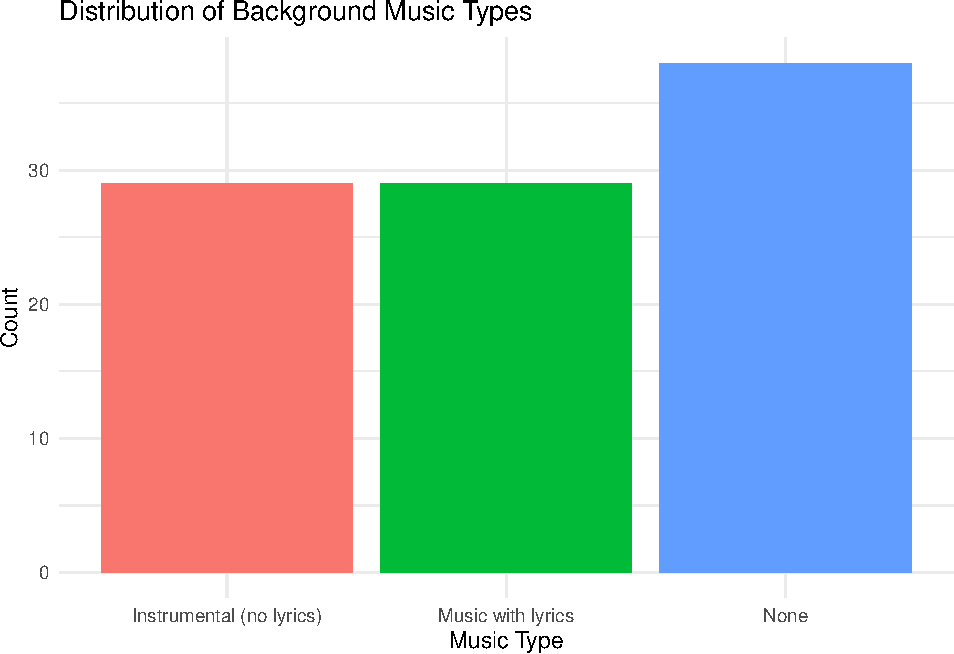
\includegraphics{Assignment2_files/figure-latex/unnamed-chunk-1-1.pdf}

This plot shows the sample size for each music type, which is important
for interpreting statistical test results later. It shows study without
music leads to heigher time to complete the task. It also shows that
type of music does not influence on the time of completion.

\subsection{Completion Time by Background Music
Type}\label{completion-time-by-background-music-type}

A boxplot visualizes TimeToComplete by MusicType to compare completion
times across music genres, providing a clear visual representation of
central tendency and spread.

\begin{Shaded}
\begin{Highlighting}[]
\FunctionTok{library}\NormalTok{(ggplot2)}
\FunctionTok{ggplot}\NormalTok{(data, }\FunctionTok{aes}\NormalTok{(}\AttributeTok{x =}\NormalTok{ MusicType, }\AttributeTok{y =}\NormalTok{ TimeToComplete, }\AttributeTok{fill =}\NormalTok{ MusicType)) }\SpecialCharTok{+}
  \FunctionTok{geom\_boxplot}\NormalTok{() }\SpecialCharTok{+}
  \FunctionTok{labs}\NormalTok{(}\AttributeTok{title =} \StringTok{"Completion Time by Background Music Type"}\NormalTok{,}
       \AttributeTok{x =} \StringTok{"Music Type"}\NormalTok{,}
       \AttributeTok{y =} \StringTok{"Time to Complete (minutes)"}\NormalTok{) }\SpecialCharTok{+}
  \FunctionTok{theme\_minimal}\NormalTok{() }\SpecialCharTok{+}
  \FunctionTok{theme}\NormalTok{(}\AttributeTok{legend.position =} \StringTok{"none"}\NormalTok{)}
\end{Highlighting}
\end{Shaded}

\begin{verbatim}
## Warning: Removed 3 rows containing non-finite outside the scale range
## (`stat_boxplot()`).
\end{verbatim}

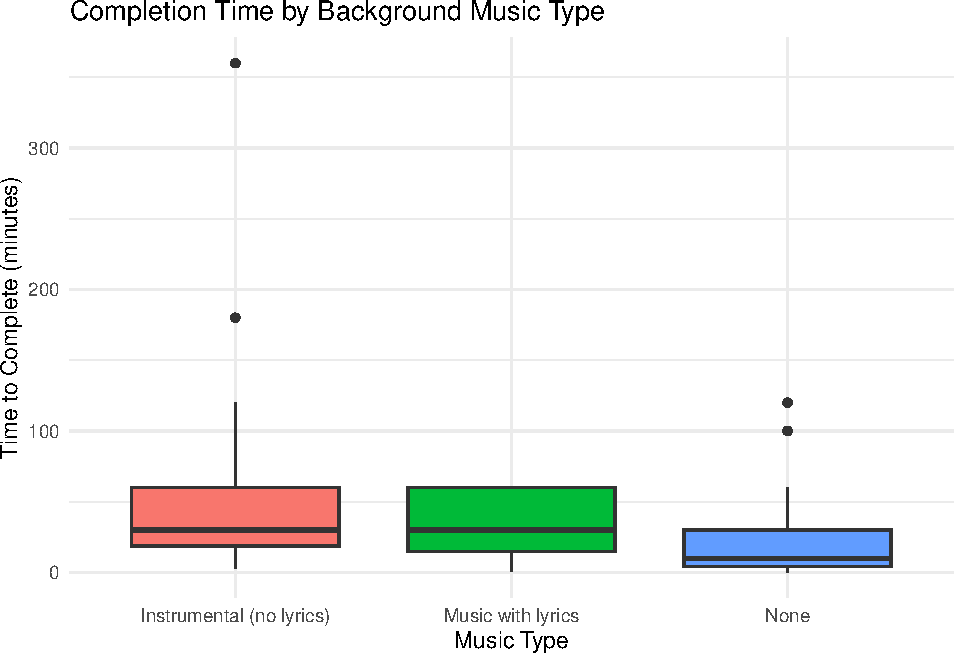
\includegraphics{Assignment2_files/figure-latex/unnamed-chunk-2-1.pdf}

according to the boxplot, when students lesten to the musice, they need
more time to complete their task. Type of music are not different a lot.

\subsection{Focus Level by Background Music
Type}\label{focus-level-by-background-music-type}

A boxplot for FocusLevel by MusicType helps visualize differences in
self-reported focus.

\begin{Shaded}
\begin{Highlighting}[]
\FunctionTok{ggplot}\NormalTok{(data, }\FunctionTok{aes}\NormalTok{(}\AttributeTok{x =}\NormalTok{ MusicType, }\AttributeTok{y =}\NormalTok{ FocusLevel, }\AttributeTok{fill =}\NormalTok{ MusicType)) }\SpecialCharTok{+}
  \FunctionTok{geom\_boxplot}\NormalTok{() }\SpecialCharTok{+}
  \FunctionTok{labs}\NormalTok{(}\AttributeTok{title =} \StringTok{"Focus Level by Background Music Type"}\NormalTok{,}
       \AttributeTok{x =} \StringTok{"Music Type"}\NormalTok{,}
       \AttributeTok{y =} \StringTok{"Focus Level (1{-}10)"}\NormalTok{) }\SpecialCharTok{+}
  \FunctionTok{theme\_minimal}\NormalTok{() }\SpecialCharTok{+}
  \FunctionTok{theme}\NormalTok{(}\AttributeTok{legend.position =} \StringTok{"none"}\NormalTok{)}
\end{Highlighting}
\end{Shaded}

\begin{verbatim}
## Warning: Removed 1 row containing non-finite outside the scale range
## (`stat_boxplot()`).
\end{verbatim}

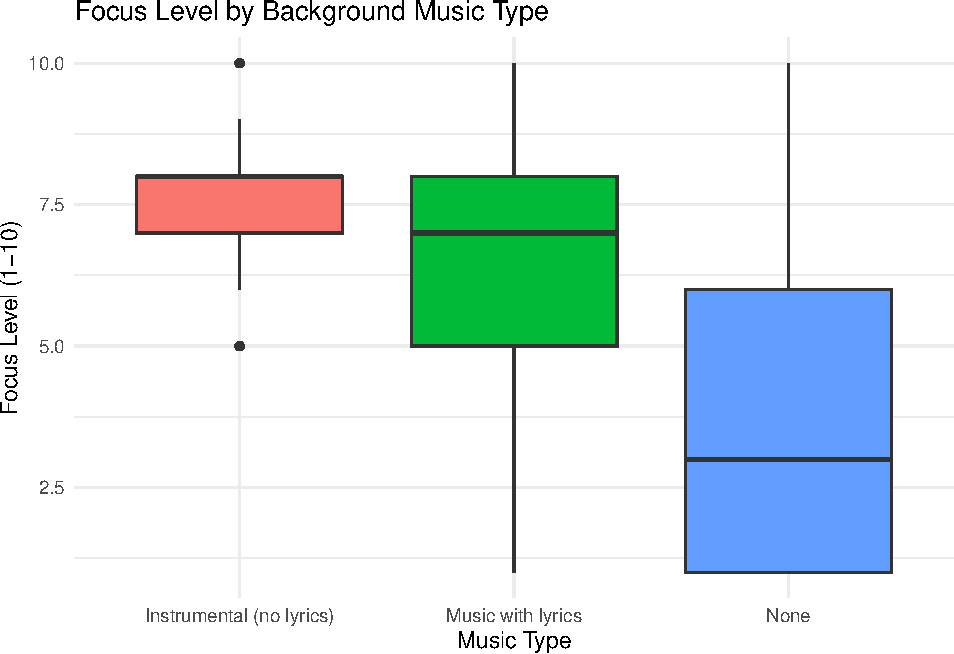
\includegraphics{Assignment2_files/figure-latex/unnamed-chunk-3-1.pdf}

This plot provides a visual comparison of focus levels across different
music types. Instrumental music appears to be associated with slightly
higher median focus levels.

\subsection{Distribution of Numerical
Variables}\label{distribution-of-numerical-variables}

Histograms for FocusLevel and TimeToComplete show their overall
distributions.

\begin{Shaded}
\begin{Highlighting}[]
\FunctionTok{library}\NormalTok{(cowplot) }\CommentTok{\# For combining plots}

\NormalTok{p1 }\OtherTok{\textless{}{-}} \FunctionTok{ggplot}\NormalTok{(data, }\FunctionTok{aes}\NormalTok{(}\AttributeTok{x =}\NormalTok{ FocusLevel)) }\SpecialCharTok{+}
  \FunctionTok{geom\_histogram}\NormalTok{(}\AttributeTok{binwidth =} \DecValTok{1}\NormalTok{, }\AttributeTok{fill =} \StringTok{"skyblue"}\NormalTok{, }\AttributeTok{color =} \StringTok{"black"}\NormalTok{) }\SpecialCharTok{+}
  \FunctionTok{labs}\NormalTok{(}\AttributeTok{title =} \StringTok{"Distribution of Focus Level"}\NormalTok{, }\AttributeTok{x =} \StringTok{"Focus Level"}\NormalTok{, }\AttributeTok{y =} \StringTok{"Count"}\NormalTok{) }\SpecialCharTok{+}
  \FunctionTok{theme\_minimal}\NormalTok{()}

\NormalTok{p2 }\OtherTok{\textless{}{-}} \FunctionTok{ggplot}\NormalTok{(data, }\FunctionTok{aes}\NormalTok{(}\AttributeTok{x =}\NormalTok{ TimeToComplete)) }\SpecialCharTok{+}
  \FunctionTok{geom\_histogram}\NormalTok{(}\AttributeTok{fill =} \StringTok{"lightgreen"}\NormalTok{, }\AttributeTok{color =} \StringTok{"black"}\NormalTok{) }\SpecialCharTok{+}
  \FunctionTok{labs}\NormalTok{(}\AttributeTok{title =} \StringTok{"Distribution of Time to Complete"}\NormalTok{, }\AttributeTok{x =} \StringTok{"Time to Complete (minutes)"}\NormalTok{, }\AttributeTok{y =} \StringTok{"Count"}\NormalTok{) }\SpecialCharTok{+}
  \FunctionTok{theme\_minimal}\NormalTok{()}

\FunctionTok{plot\_grid}\NormalTok{(p1, p2, }\AttributeTok{ncol =} \DecValTok{2}\NormalTok{)}
\end{Highlighting}
\end{Shaded}

\begin{verbatim}
## Warning: Removed 1 row containing non-finite outside the scale range
## (`stat_bin()`).
\end{verbatim}

\begin{verbatim}
## `stat_bin()` using `bins = 30`. Pick better value with `binwidth`.
\end{verbatim}

\begin{verbatim}
## Warning: Removed 3 rows containing non-finite outside the scale range
## (`stat_bin()`).
\end{verbatim}

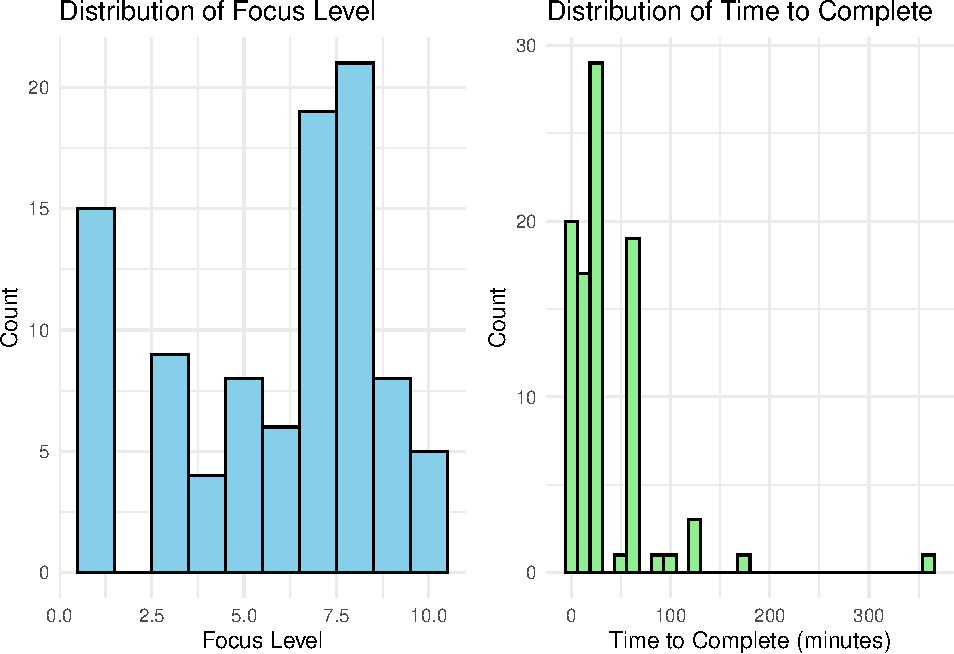
\includegraphics{Assignment2_files/figure-latex/unnamed-chunk-4-1.pdf}

These histograms provide insights into the overall spread and skewness
of the numerical variables, which is useful for assessing normality
assumptions later.

\subsection{Conclusion}\label{conclusion}

Thease diagrams can answer the questions below:

\begin{itemize}
\item
  RQ1: How does the type of music or silence influence students' focus
  levels? As the statistices calculations show, listening to the music
  has a positive influence on the focus level. But the type of the music
  does not impact on it. it shows, studing in scilence will lead to
  lower focus level. But in the future in the test we will see that
  listening to the music while studing has a negative impact and it
  caused by the outlier and noises in the data which has a negative
  impact on this visualisation.
\item
  RQ3: How does the type of background music impact the time required to
  complete a task? Type of Backgraound music does not have influce on
  it. They are same.
\end{itemize}

\section{Descriptive Inference}\label{descriptive-inference}

Summary statistics for FocusLevel and TimeToComplete are computed for
each MusicType, now presented with more detail including median and
interquartile range to complement mean and standard deviation, which are
more robust to outliers.

\begin{Shaded}
\begin{Highlighting}[]
\FunctionTok{library}\NormalTok{(knitr)}
\FunctionTok{library}\NormalTok{(dplyr)}

\NormalTok{summary\_stats }\OtherTok{\textless{}{-}}\NormalTok{ data }\SpecialCharTok{\%\textgreater{}\%}
  \FunctionTok{group\_by}\NormalTok{(MusicType) }\SpecialCharTok{\%\textgreater{}\%}
  \FunctionTok{summarise}\NormalTok{(}
    \AttributeTok{N =} \FunctionTok{n}\NormalTok{(),}
    \AttributeTok{Mean\_Focus =} \FunctionTok{mean}\NormalTok{(FocusLevel, }\AttributeTok{na.rm =} \ConstantTok{TRUE}\NormalTok{),}
    \AttributeTok{SD\_Focus =} \FunctionTok{sd}\NormalTok{(FocusLevel, }\AttributeTok{na.rm =} \ConstantTok{TRUE}\NormalTok{),}
    \AttributeTok{Median\_Focus =} \FunctionTok{median}\NormalTok{(FocusLevel, }\AttributeTok{na.rm =} \ConstantTok{TRUE}\NormalTok{),}
    \AttributeTok{IQR\_Focus =} \FunctionTok{IQR}\NormalTok{(FocusLevel, }\AttributeTok{na.rm =} \ConstantTok{TRUE}\NormalTok{),}
    \AttributeTok{Mean\_Time =} \FunctionTok{mean}\NormalTok{(TimeToComplete, }\AttributeTok{na.rm =} \ConstantTok{TRUE}\NormalTok{),}
    \AttributeTok{SD\_Time =} \FunctionTok{sd}\NormalTok{(TimeToComplete, }\AttributeTok{na.rm =} \ConstantTok{TRUE}\NormalTok{),}
    \AttributeTok{Median\_Time =} \FunctionTok{median}\NormalTok{(TimeToComplete, }\AttributeTok{na.rm =} \ConstantTok{TRUE}\NormalTok{),}
    \AttributeTok{IQR\_Time =} \FunctionTok{IQR}\NormalTok{(TimeToComplete, }\AttributeTok{na.rm =} \ConstantTok{TRUE}\NormalTok{)}
\NormalTok{  )}

\FunctionTok{print}\NormalTok{(summary\_stats)}
\end{Highlighting}
\end{Shaded}

\begin{verbatim}
## # A tibble: 3 x 10
##   MusicType       N Mean_Focus SD_Focus Median_Focus IQR_Focus Mean_Time SD_Time
##   <fct>       <int>      <dbl>    <dbl>        <dbl>     <dbl>     <dbl>   <dbl>
## 1 Instrument~    29       7.79     1.15            8         1      52.6    71.2
## 2 Music with~    29       6.72     2.15            7         3      33.1    21.6
## 3 None           38       3.68     2.69            3         5      24.2    32.9
## # i 2 more variables: Median_Time <dbl>, IQR_Time <dbl>
\end{verbatim}

The enhanced table confirms that instrumental music has slightly higher
mean/median focus levels and lower mean/median completion times. The IQR
gives a better sense of data spread compared to just standard deviation.

\section{ANOVA}\label{anova}

We check the normality of the residuals from the ANOVA model. This can
be done visually with a QQ plot.

\begin{Shaded}
\begin{Highlighting}[]
\FunctionTok{library}\NormalTok{(car)    }
\end{Highlighting}
\end{Shaded}

\begin{verbatim}
## Loading required package: carData
\end{verbatim}

\begin{verbatim}
## 
## Attaching package: 'car'
\end{verbatim}

\begin{verbatim}
## The following object is masked from 'package:dplyr':
## 
##     recode
\end{verbatim}

\begin{Shaded}
\begin{Highlighting}[]
\CommentTok{\# Build the linear model for ANOVA}
\NormalTok{anova\_model }\OtherTok{\textless{}{-}} \FunctionTok{aov}\NormalTok{(TimeToComplete }\SpecialCharTok{\textasciitilde{}}\NormalTok{ MusicType, }\AttributeTok{data =}\NormalTok{ data)}

\CommentTok{\# QQ plot of residuals}
\FunctionTok{plot}\NormalTok{(anova\_model,}\DecValTok{2}\NormalTok{) }
\FunctionTok{title}\NormalTok{(}\StringTok{"QQ Plot of Residuals"}\NormalTok{)}
\end{Highlighting}
\end{Shaded}

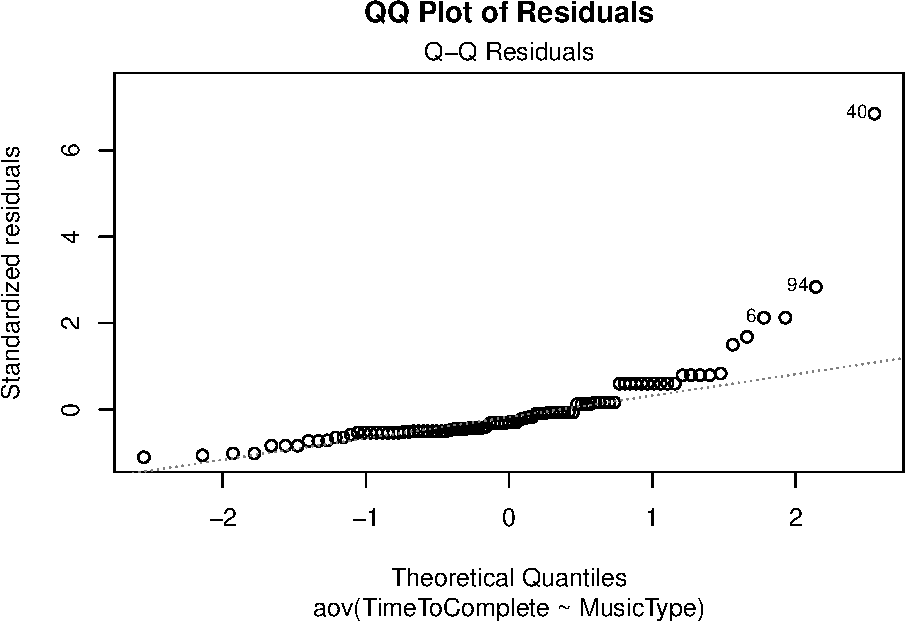
\includegraphics{Assignment2_files/figure-latex/unnamed-chunk-6-1.pdf}

\begin{Shaded}
\begin{Highlighting}[]
\FunctionTok{print}\NormalTok{(anova\_model)}
\end{Highlighting}
\end{Shaded}

\begin{verbatim}
## Call:
##    aov(formula = TimeToComplete ~ MusicType, data = data)
## 
## Terms:
##                 MusicType Residuals
## Sum of Squares    12969.5  187906.5
## Deg. of Freedom         2        90
## 
## Residual standard error: 45.693
## Estimated effects may be unbalanced
## 3 observations deleted due to missingness
\end{verbatim}

\begin{Shaded}
\begin{Highlighting}[]
\FunctionTok{library}\NormalTok{(car)    }

\CommentTok{\# Build the linear model for ANOVA}
\NormalTok{anova\_model\_focous }\OtherTok{\textless{}{-}} \FunctionTok{aov}\NormalTok{(FocusLevel }\SpecialCharTok{\textasciitilde{}}\NormalTok{ MusicType, }\AttributeTok{data =}\NormalTok{ data)}

\CommentTok{\# QQ plot of residuals}
\FunctionTok{plot}\NormalTok{(anova\_model\_focous,}\DecValTok{2}\NormalTok{) }
\FunctionTok{title}\NormalTok{(}\StringTok{"QQ Plot of Residuals"}\NormalTok{)}
\end{Highlighting}
\end{Shaded}

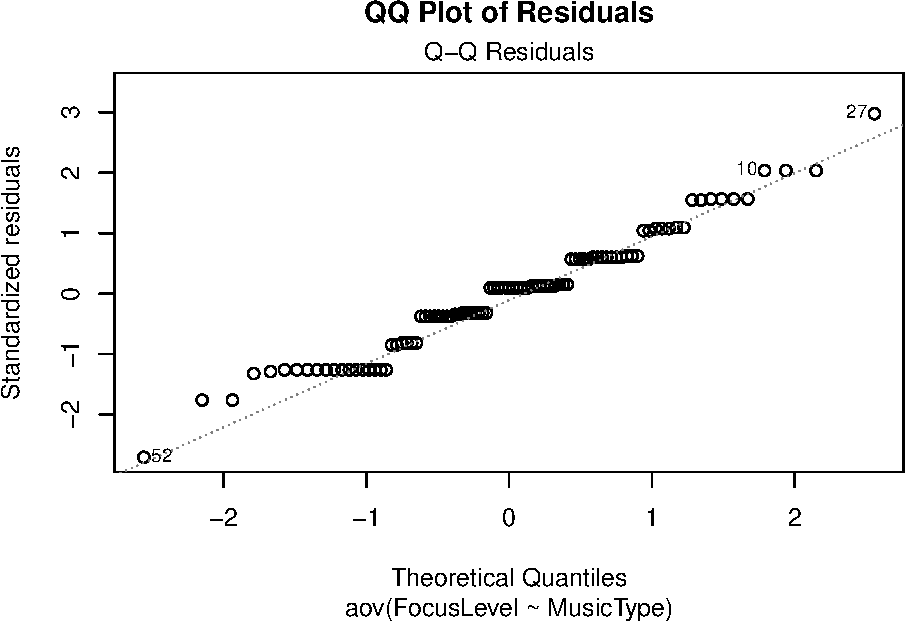
\includegraphics{Assignment2_files/figure-latex/unnamed-chunk-8-1.pdf}

\begin{Shaded}
\begin{Highlighting}[]
\FunctionTok{print}\NormalTok{(anova\_model\_focous)}
\end{Highlighting}
\end{Shaded}

\begin{verbatim}
## Call:
##    aov(formula = FocusLevel ~ MusicType, data = data)
## 
## Terms:
##                 MusicType Residuals
## Sum of Squares   306.5612  426.6598
## Deg. of Freedom         2        92
## 
## Residual standard error: 2.15351
## Estimated effects may be unbalanced
## 1 observation deleted due to missingness
\end{verbatim}

The QQ plot shows that the residuals deviate from the straight line,
especially in the upper tail, indicating a violation of the normality
assumption. This suggests the residuals are not normally distributed,
which can affect the reliability of the ANOVA results. The ANOVA table
shows that the between-group variation (MusicType) is relatively small
compared to the residual variance.

\subsection{Performing ANOVA}\label{performing-anova}

\begin{Shaded}
\begin{Highlighting}[]
\FunctionTok{library}\NormalTok{(broom) }
\NormalTok{summary\_anova }\OtherTok{\textless{}{-}} \FunctionTok{summary}\NormalTok{(anova\_model)}

\CommentTok{\# Displaying ANOVA results}
\FunctionTok{kable}\NormalTok{(}\FunctionTok{tidy}\NormalTok{(anova\_model), }\AttributeTok{caption =} \StringTok{"ANOVA Results for Completion Time by Music Type"}\NormalTok{,}
             \AttributeTok{format =} \StringTok{"latex"}\NormalTok{, }\AttributeTok{booktabs =} \ConstantTok{TRUE}\NormalTok{, }\AttributeTok{digits =} \DecValTok{3}\NormalTok{)}
\end{Highlighting}
\end{Shaded}

\begin{table}

\caption{\label{tab:unnamed-chunk-10}ANOVA Results for Completion Time by Music Type}
\centering
\begin{tabular}[t]{lrrrrr}
\toprule
term & df & sumsq & meansq & statistic & p.value\\
\midrule
MusicType & 2 & 12969.5 & 6484.75 & 3.106 & 0.05\\
Residuals & 90 & 187906.5 & 2087.85 & NA & NA\\
\bottomrule
\end{tabular}
\end{table}

\begin{Shaded}
\begin{Highlighting}[]
\CommentTok{\# Post{-}hoc test if overall ANOVA is significant}
\ControlFlowTok{if}\NormalTok{ (summary\_anova[[}\DecValTok{1}\NormalTok{]][[}\StringTok{"Pr(\textgreater{}F)"}\NormalTok{]][}\DecValTok{1}\NormalTok{] }\SpecialCharTok{\textless{}} \FloatTok{0.05}\NormalTok{) \{}
  \FunctionTok{message}\NormalTok{(}\StringTok{"Performing TukeyHSD post{-}hoc test due to significant ANOVA result:"}\NormalTok{)}
\NormalTok{  tukey\_result }\OtherTok{\textless{}{-}} \FunctionTok{TukeyHSD}\NormalTok{(anova\_model)}
  \FunctionTok{print}\NormalTok{(tukey\_result)}
\NormalTok{\} }\ControlFlowTok{else}\NormalTok{ \{}
  \FunctionTok{message}\NormalTok{(}\StringTok{"ANOVA not significant, no post{-}hoc test needed."}\NormalTok{)}
\NormalTok{\}}
\end{Highlighting}
\end{Shaded}

\begin{verbatim}
## Performing TukeyHSD post-hoc test due to significant ANOVA result:
\end{verbatim}

\begin{verbatim}
##   Tukey multiple comparisons of means
##     95% family-wise confidence level
## 
## Fit: aov(formula = TimeToComplete ~ MusicType, data = data)
## 
## $MusicType
##                                                 diff       lwr        upr
## Music with lyrics-Instrumental (no lyrics) -19.55542 -48.40580  9.2949624
## None-Instrumental (no lyrics)              -28.41270 -55.85066 -0.9747357
## None-Music with lyrics                      -8.85728 -36.02784 18.3132791
##                                                p adj
## Music with lyrics-Instrumental (no lyrics) 0.2444661
## None-Instrumental (no lyrics)              0.0406499
## None-Music with lyrics                     0.7181424
\end{verbatim}

The ANOVA tests whether mean completion times differ significantly
across music types. A p-value less than 0.05 indicates a statistically
significant difference among group means. If significant, the TukeyHSD
post-hoc test identifies which specific pairs of music types have
significantly different mean completion times. But this results are not
reliable. We perform another test.

\subsection{Kruskal-Wallis Rank Sum
Test}\label{kruskal-wallis-rank-sum-test}

If the assumptions for ANOVA are violated, the Kruskal-Wallis rank sum
test is a non-parametric alternative. It tests if there are significant
differences in the medians among groups.

\begin{Shaded}
\begin{Highlighting}[]
\CommentTok{\# Kruskal{-}Wallis Rank Sum Test}
\NormalTok{kruskal\_result }\OtherTok{\textless{}{-}} \FunctionTok{kruskal.test}\NormalTok{(TimeToComplete }\SpecialCharTok{\textasciitilde{}}\NormalTok{ MusicType, }\AttributeTok{data =}\NormalTok{ data)}
\FunctionTok{print}\NormalTok{(kruskal\_result)}
\end{Highlighting}
\end{Shaded}

\begin{verbatim}
## 
##  Kruskal-Wallis rank sum test
## 
## data:  TimeToComplete by MusicType
## Kruskal-Wallis chi-squared = 11.543, df = 2, p-value = 0.003116
\end{verbatim}

\begin{Shaded}
\begin{Highlighting}[]
\CommentTok{\# If significant, conduct Dunn\textquotesingle{}s test for post{-}hoc analysis (requires DescTools package)}
\CommentTok{\# Make sure DescTools is installed: install.packages("DescTools")}
\FunctionTok{library}\NormalTok{(DescTools)}
\end{Highlighting}
\end{Shaded}

\begin{verbatim}
## 
## Attaching package: 'DescTools'
\end{verbatim}

\begin{verbatim}
## The following object is masked from 'package:car':
## 
##     Recode
\end{verbatim}

\begin{Shaded}
\begin{Highlighting}[]
\ControlFlowTok{if}\NormalTok{ (kruskal\_result}\SpecialCharTok{$}\NormalTok{p.value }\SpecialCharTok{\textless{}} \FloatTok{0.05}\NormalTok{) \{}
  \FunctionTok{message}\NormalTok{(}\StringTok{"Performing Dunn\textquotesingle{}s post{-}hoc test due to significant Kruskal{-}Wallis result:"}\NormalTok{)}
\NormalTok{  dunn\_result }\OtherTok{\textless{}{-}}\NormalTok{ DescTools}\SpecialCharTok{::}\FunctionTok{DunnTest}\NormalTok{(TimeToComplete }\SpecialCharTok{\textasciitilde{}}\NormalTok{ MusicType, }\AttributeTok{data =}\NormalTok{ data, }\AttributeTok{method=}\StringTok{"bonferroni"}\NormalTok{)}
  \FunctionTok{print}\NormalTok{(dunn\_result)}
\NormalTok{\}}
\end{Highlighting}
\end{Shaded}

\begin{verbatim}
## Performing Dunn's post-hoc test due to significant Kruskal-Wallis result:
\end{verbatim}

\begin{verbatim}
## 
##  Dunn's test of multiple comparisons using rank sums : bonferroni  
## 
##                                            mean.rank.diff   pval    
## Music with lyrics-Instrumental (no lyrics)      -4.662562 1.0000    
## None-Instrumental (no lyrics)                  -21.339286 0.0046 ** 
## None-Music with lyrics                         -16.676724 0.0372 *  
## ---
## Signif. codes:  0 '***' 0.001 '**' 0.01 '*' 0.05 '.' 0.1 ' ' 1
\end{verbatim}

There is a significant effect of music type on task completion time.
Specifically, working without music results in faster performance than
working with either type of music (instrumental or with lyrics).
However, the type of music (instrumental vs.~lyrical) does not
significantly affect performance between each other.

\begin{Shaded}
\begin{Highlighting}[]
\CommentTok{\# Kruskal{-}Wallis Rank Sum Test}
\NormalTok{kruskal\_result\_Focous }\OtherTok{\textless{}{-}} \FunctionTok{kruskal.test}\NormalTok{(FocusLevel }\SpecialCharTok{\textasciitilde{}}\NormalTok{ MusicType, }\AttributeTok{data =}\NormalTok{ data)}
\FunctionTok{print}\NormalTok{(kruskal\_result\_Focous)}
\end{Highlighting}
\end{Shaded}

\begin{verbatim}
## 
##  Kruskal-Wallis rank sum test
## 
## data:  FocusLevel by MusicType
## Kruskal-Wallis chi-squared = 36.405, df = 2, p-value = 1.244e-08
\end{verbatim}

\begin{Shaded}
\begin{Highlighting}[]
\CommentTok{\# If significant, conduct Dunn\textquotesingle{}s test for post{-}hoc analysis (requires DescTools package)}
\CommentTok{\# Make sure DescTools is installed: install.packages("DescTools")}
\FunctionTok{library}\NormalTok{(DescTools)}
\ControlFlowTok{if}\NormalTok{ (kruskal\_result\_Focous}\SpecialCharTok{$}\NormalTok{p.value }\SpecialCharTok{\textless{}} \FloatTok{0.05}\NormalTok{) \{}
  \FunctionTok{message}\NormalTok{(}\StringTok{"Performing Dunn\textquotesingle{}s post{-}hoc test due to significant Kruskal{-}Wallis result:"}\NormalTok{)}
\NormalTok{  dunn\_result\_Focous }\OtherTok{\textless{}{-}}\NormalTok{ DescTools}\SpecialCharTok{::}\FunctionTok{DunnTest}\NormalTok{(FocusLevel }\SpecialCharTok{\textasciitilde{}}\NormalTok{ MusicType, }\AttributeTok{data =}\NormalTok{ data, }\AttributeTok{method=}\StringTok{"bonferroni"}\NormalTok{)}
  \FunctionTok{print}\NormalTok{(dunn\_result\_Focous)}
\NormalTok{\}}
\end{Highlighting}
\end{Shaded}

\begin{verbatim}
## Performing Dunn's post-hoc test due to significant Kruskal-Wallis result:
\end{verbatim}

\begin{verbatim}
## 
##  Dunn's test of multiple comparisons using rank sums : bonferroni  
## 
##                                            mean.rank.diff    pval    
## Music with lyrics-Instrumental (no lyrics)      -11.75862 0.29991    
## None-Instrumental (no lyrics)                   -39.12488   2e-08 ***
## None-Music with lyrics                          -27.36626 0.00015 ***
## ---
## Signif. codes:  0 '***' 0.001 '**' 0.01 '*' 0.05 '.' 0.1 ' ' 1
\end{verbatim}

The Kruskal-Wallis rank sum test revealed a significant difference in
FocusLevel across different MusicType categories, with a p-value of
1.244e-08, indicating that the type of music affects focus levels.
Dunn's post-hoc test with Bonferroni correction further clarified that
there is no significant difference between music with lyrics and
instrumental music (p = 0.29991), but significant differences exist
between instrumental music and no music (p = 2e-08) as well as between
music with lyrics and no music (p = 0.00015). These findings suggest
that the presence of music, regardless of whether it includes lyrics,
impacts focus levels differently compared to the absence of music. The
negative mean rank differences imply that focus levels tend to be lower
when music is present compared to no music, though the exact magnitude
depends on the specific context of the data. Overall, this analysis
highlights that eliminating music may enhance focus.

\textbackslash{} The mean FocusLevel appears higher with music compared
to no music in the summary statistics, yet the Kruskal-Wallis and Dunn's
tests suggest lower focus with music. The summary statistics indicate
higher mean and median FocusLevel for ``Instrumental'' and ``Music with
lyrics'' compared to ``None,'' which aligns with the boxplot observation
(Section 3.3) of slightly higher median focus with instrumental music.
However, the Kruskal-Wallis test on FocusLevel and the subsequent Dunn's
post-hoc test reveal a significant difference, with negative mean rank
differences (-39.12488 for None vs.~Instrumental, p = 2e-08; -27.36626
for None vs.~Music with lyrics, p = 0.00015), indicating that FocusLevel
is significantly lower when music is present compared to no music,
despite the higher means.

This apparent contradiction arises because the mean and median values
reflect central tendencies that can be influenced by the distribution's
shape, while the Kruskal-Wallis test and Dunn's test assess differences
in ranks, which are less sensitive to the exact scale but highlight
relative ordering. The histograms and the QQ plot for the ANOVA
residuals suggest non-normal distributions and potential outliers, which
could explain why the mean FocusLevel is higher with music , while the
rank-based tests indicate lower focus relative to ``None.'' The Dunn's
test shows no significant difference between ``Instrumental'' and
``Music with lyrics'' (p = 0.29991), consistent with the summary
statistics' close means, but the significant drop in rank for music
groups versus ``None'' suggests that self-reported focus is lower in the
presence of music when considering the entire distribution.

\subsection{Effect of MusicType and FocusLevel on Time to
Complete}\label{effect-of-musictype-and-focuslevel-on-time-to-complete}

\begin{Shaded}
\begin{Highlighting}[]
\NormalTok{anova\_model }\OtherTok{\textless{}{-}} \FunctionTok{aov}\NormalTok{(TimeToComplete }\SpecialCharTok{\textasciitilde{}}\NormalTok{ MusicType }\SpecialCharTok{*}\NormalTok{ FocusLevel, }\AttributeTok{data =}\NormalTok{ data)}
\FunctionTok{summary}\NormalTok{(anova\_model)}
\end{Highlighting}
\end{Shaded}

\begin{verbatim}
##                      Df Sum Sq Mean Sq F value Pr(>F)  
## MusicType             2  12969    6485   3.337 0.0401 *
## FocusLevel            1     59      59   0.030 0.8623  
## MusicType:FocusLevel  2  18804    9402   4.839 0.0102 *
## Residuals            87 169043    1943                 
## ---
## Signif. codes:  0 '***' 0.001 '**' 0.01 '*' 0.05 '.' 0.1 ' ' 1
## 3 observations deleted due to missingness
\end{verbatim}

But Here we use Scheirer-Ray-Hare test, an extension of the
Kruskal-Wallis test for two-way designs. This test analyzes the main
effects and interaction using ranks, making it appropriate for
non-normal data.

\begin{Shaded}
\begin{Highlighting}[]
\FunctionTok{library}\NormalTok{(rcompanion)}
\NormalTok{rh\_result }\OtherTok{\textless{}{-}} \FunctionTok{scheirerRayHare}\NormalTok{(TimeToComplete }\SpecialCharTok{\textasciitilde{}}\NormalTok{ MusicType }\SpecialCharTok{*}\NormalTok{ FocusLevel, }\AttributeTok{data =}\NormalTok{ data)}
\end{Highlighting}
\end{Shaded}

\begin{verbatim}
## 
## DV:  TimeToComplete 
## Observations:  93 
## D:  0.9808123 
## MS total:  728.5
\end{verbatim}

\begin{Shaded}
\begin{Highlighting}[]
\FunctionTok{print}\NormalTok{(rh\_result)}
\end{Highlighting}
\end{Shaded}

\begin{verbatim}
##                      Df Sum Sq      H p.value
## MusicType             2   3718 5.2037 0.07414
## FocusLevel            8   6599 9.2349 0.32287
## MusicType:FocusLevel 11   5670 7.9357 0.71906
## Residuals            71  45220
\end{verbatim}

RQ3: How does the type of background music impact the time required to
complete a task?

The Scheirer-Ray-Hare test showed no statistically significant effects
overall. MusicType had a marginal effect on TimeToComplete (p = 0.074),
suggesting a possible influence, though not significant at the 0.05
level. FocusLevel (p = 0.323) and the interaction between MusicType and
FocusLevel (p = 0.719) were not significant. This suggests that neither
focus level nor its combination with music type had a clear impact on
task completion time

\section{Functions}\label{functions}

\begin{verbatim}
read_excel(): Imports data from an Excel file into an R data frame.

rename(): Changes column names in a data frame. 

filter(): Subsets rows in a data frame based on specified conditions. 

as.numeric(): Converts a variable to numeric type. 

gsub(): Replaces specific patterns in text strings with new values. 

as.factor(): Converts a variable to a factor. 

ggplot(): Initializes a plot object for creating customizable visualizations. 

geom_bar(): Creates a bar plot to display counts or summaries of categorical data. 

geom_boxplot(): Generates a boxplot to show the distribution and spread of data. 

labs(): Adds or modifies titles, axis labels, and other annotations in plots. 

theme_minimal(): Applies a clean, minimalistic theme to ggplot visualizations. 

geom_histogram(): Plots a histogram to visualize the distribution of a variable. 

plot_grid(): Arranges multiple plots into a single grid for combined display. 

group_by(): Groups data by one or more variables for aggregated analysis. 

summarise(): Computes summary statistics for grouped data. 

IQR(): Calculates the interquartile range of a numeric vector. 

kable(): Formats data frames or matrices into tables for reports. 

aov(): Fits an analysis of variance (ANOVA) model to compare group means. 

plot(): Creates diagnostic plots, such as QQ plots, for model evaluation. 

summary(): Provides a summary of statistical model results or data. 

tidy(): Converts model outputs into a tidy data frame for easier handling. 

TukeyHSD(): Performs post-hoc pairwise comparisons for ANOVA results. 

kruskal.test(): Conducts a non-parametric test to compare medians across groups. 

DunnTest(): Performs post-hoc pairwise comparisons for non-parametric tests.
\end{verbatim}

\end{document}
